\documentclass[11pt]{article}

\usepackage[margin=1in]{geometry}
\usepackage{amsmath,amssymb,amsthm}
\usepackage{graphicx}
\usepackage{booktabs}
\usepackage{xcolor}
\usepackage[numbers,sort&compress]{natbib}
\usepackage[colorlinks=true,linkcolor=black,citecolor=blue,urlcolor=blue]{hyperref}

\graphicspath{{figures/}}
\setlength{\emergencystretch}{2em}
\newcommand{\IC}{\mathrm{IC}}

\title{\bfseries How Much Does Purging Actually Fix?\\
A Controlled Quantification of Overlap Leakage\\ in Time-Series Cross-Validation}

\author{Eugen Soloviov\thanks{Independent Researcher. ORCID:
\href{https://orcid.org/0009-0006-3148-111X}{0009-0006-3148-111X}.
Correspondence: \href{mailto:suenot@gmail.com}{suenot@gmail.com}.
Code to reproduce every number and figure:
\url{https://github.com/suenot/purged-cv-leakage}.}}

\date{}

\begin{document}
\maketitle

\begin{abstract}
Financial machine learning teaches that $k$-fold cross-validation ``fails in
finance'' because forward-looking labels overlap, and prescribes purged
$k$-fold CV with an embargo as the remedy; the forecasting literature proves,
to the contrary, that standard $k$-fold CV is valid for autoregressive
prediction. We reconcile the two in a controlled simulation in which true
predictability is known exactly---including exactly zero---and leakage is
measured directly as the CV estimate minus the true forward skill of the same
fitted models. Under the null, the phantom skill of naive shuffled $k$-fold is
an \emph{interaction} of two ingredients. With $h$-period overlapping labels
\emph{and} persistent features (AR(1), $\phi=0.97$), a random forest reports a
cross-validated information coefficient of $+0.31$/$+0.46$/$+0.56$ ($\pm0.05$)
at $h=5/10/20$ where the truth is zero (ridge $+0.18\pm0.04$; classification
AUC $0.623$ reported vs.\ $0.504$ true, $+0.119\pm0.010$). Remove either
ingredient and the phantom vanishes---at most $+0.005$ at $h=1$ for any
$\phi$, and at most $+0.005$ at $\phi=0$ for any $h$---exactly the regimes the
validity results describe. Decomposing the remedy: \emph{blocked} (contiguous)
$k$-fold without any purging already removes nearly all of the \emph{mean}
bias (residual $-0.05\pm0.04$ at the worst-leakage cell); at $h \ll T$ purging
buys the worst-case guarantee, not the average. Purged $k$-fold leaves no
residual optimism at \emph{zero} embargo in all ten arms tested (five
signal-persistence arms $\times$ two models, persistence up to
$0.995$); the residual is negative ($-0.010$ to $-0.102$ under the
pooled-prediction scoring convention, a contiguous-fold
pessimism) and flat across the embargo grid---the embargo bought nothing in
this design, whose features are exogenous; the return-derived-feature case
that motivates embargoes is explicitly out of scope. The costs are modest:
purging discards $1.2$--$1.3\%$ of training candidates (by batch geometry)
and CV dispersion rises
$21\%$ ($0.048 \to 0.058$), almost all of it from contiguity rather than from
the purge itself; walk-forward keeps $72.7\%$ of the data with twice the
fold-level dispersion. The payoff is model selection: with a genuine signal
(population IC $0.100$), naive CV selects the leakage-maximizing $k$NN in
$50$ of $50$ repetitions (claimed IC $0.422$, true $0.012$; optimism
$+0.410$), while purged CV selects honestly (optimism $+0.012$), lifting the
true forward IC of the deployed model from $0.012$ to $0.042$---a gain of
$+0.029\pm0.012$ (wins $64\%$, ties $18\%$; oracle $0.069$).
\end{abstract}

\section{Introduction}

When the label of a financial prediction problem is a forward $h$-period
return, consecutive training samples share $h-1$ of their $h$ label returns.
\citet{lopezdeprado2018advances} argues that this overlap leaks information
between cross-validation folds, inflates measured performance, and is one
reason backtested strategies fail in production; his prescription---purged
$k$-fold cross-validation with an embargo---has become standard practice in
financial machine learning, shipped in widely used open-source libraries and
adopted essentially on textbook authority. The supporting evidence, however,
is illustrative rather than quantitative: how large the bias actually is, what
data properties control it, and how much of it each component of the remedy
(contiguous folds, purging, embargo) removes have not been measured.

The question is sharper than it looks, because a neighboring literature says
the opposite. \citet{bergmeir2018note} prove that standard $k$-fold
cross-validation is \emph{valid} for purely autoregressive prediction with
uncorrelated errors, and empirical comparisons
\citep{bergmeir2012use,cerqueira2020evaluating} repeatedly find vanilla or
blocked CV competitive with the out-of-sample evaluations
\citep{tashman2000out} that practitioners trust. If naive CV is provably fine
for time series in those settings, the case for aggressive purging must rest
on a specific mechanism that those settings lack---and identifying that
mechanism is a prerequisite for knowing when purging is necessary, when it is
harmless insurance, and when it wastes data.

This paper measures the mechanism directly.\footnote{The splitting procedures
under test, including the specific purge-and-embargo construction we
implement, follow the author's own earlier practitioner explainer on purged
cross-validation (a \mbox{marketmaker.cc} article). The present paper is a
controlled self-audit of advice the author has himself circulated, not an
attack on a third party.} We build a simulation in which the true
predictability of every feature is known exactly---including the case of
exactly zero---and define leakage operationally: the cross-validated skill
estimate minus the true forward skill of the very same fitted models,
measured on an untouched continuation of the series. Because the truth is
known, ``phantom skill'' is not an interpretation but a number, with a
confidence interval, as a function of the label horizon $h$ and the feature
persistence $\phi$.

The headline result is an interaction that reconciles the two literatures.
Overlap alone does not create phantom skill: with serially independent
features, naive shuffled $k$-fold shows no optimistic bias in IC at any
horizon we test.
Persistence alone does not create it either: with non-overlapping labels
($h=1$), even features with $\phi=0.97$ produce nothing. The leak requires
the \emph{product}: a persistent feature lets the model locate a test
sample's temporal neighbors in feature space, and the overlapping label tells
it what those neighbors' labels (mostly) were. Autoregressive setups of the
Bergmeir line live on the two harmless axes; $h$-period forward labels with
persistent predictors---the standard financial configuration---live in the
interaction region, where we measure phantom information coefficients up to
$+0.56$ for a random forest under a null with exactly zero true signal. Both
literatures are right in their own regime, and the boundary between the
regimes is the product of overlap and persistence.

Measuring the remedy against the same ground truth produces three findings
that practitioners may find uncomfortable in opposite directions. First,
\emph{blocked} $k$-fold---contiguous test blocks, no purging at all---already
removes nearly all of the mean bias; at $h \ll T$, purging's marginal
contribution to calibration is second-order, and what it actually buys is the
worst case (zero overlapping pairs by construction), not the average. Second,
the \emph{embargo} bought nothing anywhere in our design: purged $k$-fold is
already calibrated at zero embargo in every arm, including genuine signals
with persistence up to $0.995$, and the embargo sweep is flat. We are explicit
about scope: our features are exogenous AR(1) processes, and the case the
embargo exists for---features \emph{derived from} past returns, whose serial
dependence echoes the label beyond the overlap window---is deliberately out of
scope here. Third, the place where purging pays unambiguously is
\emph{model selection}: scored by naive CV, the model menu is ranked by
leakage-harvesting ability rather than true skill, and the worst true model
wins every time; scored by purged CV, the truly best model wins most often,
and the deployed skill more than triples.

\paragraph{Contributions.}
\begin{enumerate}\itemsep2pt
\item A reproducible known-truth framework for leakage measurement: a
data-generating process with overlapping forward labels and AR(1) features
whose population information coefficient is available in closed form
(including exactly zero); a forward-truth protocol that scores each fold's
fitted model on an untouched continuation separated by an $h$-step gap; and
from-scratch splitter implementations whose zero-overlap property is verified
by an exhaustive train/test pair checker (Sections~\ref{sec:splitters}--\ref{sec:framework}).
\item A quantification of phantom skill under the null as a function of
$(h,\phi)$, showing it is an interaction---absent at $h=1$ for any $\phi$ and
at $\phi=0$ for any $h$, up to $+0.564\pm0.048$ IC when both are present---and
model-dependent (random forest absorbs roughly three times more of the leak
than ridge; the same pattern holds for classification AUC). This measurement
offers, to our knowledge, the first joint account of the
\citet{bergmeir2018note} validity results and the financial-ML failure
mode---by analogy rather than replication: the Bergmeir-line experiments use
endogenous lagged-target features, a class our embargo discussion declares
out of scope, so we explain \emph{why} their settings sit on the harmless
axes rather than re-run them (Section~\ref{sec:interaction}).
\item A decomposition of the remedy: contiguous blocks alone remove nearly all
mean bias; purging adds the worst-case guarantee at a $1.2\%$ data cost; the
embargo adds nothing for exogenous features, a deliberately disclosed negative
result (Sections~\ref{sec:blocking}--\ref{sec:embargo}).
\item A cost accounting---training data discarded, CV-estimate dispersion,
walk-forward's data efficiency---showing the dispersion price of the honest
procedure comes from contiguity, not from the purge
(Section~\ref{sec:costs}).
\item A demonstration that the bias becomes a wrong \emph{decision} at the
model-selection stage, and that purged CV repairs the decision, not just the
estimate: true forward IC of the selected model $0.012 \to 0.042$ against an
oracle of $0.069$ (Section~\ref{sec:selection}).
\end{enumerate}

\section{Related work}
\label{sec:related}

\paragraph{Cross-validation under dependence.} The difficulties serial
dependence creates for cross-validation were identified long before financial
machine learning popularized them. \citet{burman1994crossvalidatory}
introduced $h$-block cross-validation, deleting the $h$ observations on
either side of each test point so that the training set is approximately
independent of it, and \citet{racine2000consistent} extended this to
$hv$-block cross-validation, additionally removing a contiguous validation
block and proving consistency of model selection for general stationary
processes. Both constructions are direct ancestors of the purging-and-embargo
procedure now standard in finance, yet neither paper quantifies how much
optimistic bias the deleted observations would otherwise contribute for a
given dependence structure---$h$ is treated as a tuning constant, not a
measured requirement. The broader theory of cross-validation, including its
known failure modes, is surveyed by \citet{arlot2010survey}, who note that
the i.i.d.\ assumption is load-bearing for most risk-estimation guarantees
and that corrections for dependent data remain comparatively underdeveloped.

\paragraph{Evaluation protocols for time-series prediction.} In forecasting,
the default response to dependence has been out-of-sample (walk-forward)
evaluation \citep{tashman2000out}. \citet{bergmeir2012use} compared blocked
and standard cross-validation against out-of-sample evaluation across
simulated and real series and found, perhaps surprisingly, that
cross-validation variants were competitive and often preferable on efficiency
grounds. \citet{bergmeir2018note} sharpened this into a theoretical result:
for purely autoregressive models with uncorrelated errors, standard $k$-fold
cross-validation is \emph{valid}---the feared temporal leakage does not
materialize. Large-scale comparisons by \citet{cerqueira2020evaluating}
complicate the picture further, finding that the best protocol depends on
series length and stationarity. This line of work sits in unresolved tension
with financial practice: if naive cross-validation is provably fine in
autoregressive settings, the case for aggressive purging must rest on a
specific leakage mechanism---and that mechanism, we show, is the overlapping
forward-return label \emph{combined with} persistent features, not
autocorrelation of the target per se. Our controlled design isolates exactly
that combination and maps the boundary between the two regimes.

\paragraph{Purging, embargo, and backtest overfitting in finance.}
\citet{lopezdeprado2018advances} gives the canonical statement of the problem
in financial machine learning: when labels are computed from forward windows
of returns, observations whose label intervals overlap leak information
between training and test folds, inflating measured performance; his
Chapter~7 prescribes purged $k$-fold cross-validation with an embargo as the
remedy. The prescription has been adopted essentially on textbook
authority---implementations ship in widely used open-source backtesting
libraries---but the supporting evidence is illustrative rather than
quantitative. Closely related is the literature on backtest overfitting:
\citet{bailey2014pseudo} showed how multiple testing over strategy
configurations manufactures spurious Sharpe ratios, and
\citet{bailey2017probability} operationalized this as the probability of
backtest overfitting, estimated via combinatorially symmetric
cross-validation. \citet{hansen2012choice} document a complementary channel,
the mining of the in-sample/out-of-sample split point itself. These papers
quantify \emph{selection-induced} phantom skill; none measures the
\emph{split-induced} phantom skill that purging targets, nor how the two
interact when leaky validation scores feed a model-selection step---the
interaction our Section~\ref{sec:selection} measures directly.

\paragraph{Leakage as a general ML failure mode.} Outside finance,
\citet{kaufman2012leakage} provided the standard formulation of leakage in
data mining: the use of information at training time that would be
illegitimately unavailable at deployment. \citet{hammerla2015lets}
demonstrated a structurally identical phenomenon in activity recognition,
where similarity between temporally adjacent windowed records biases
cross-validation upward, and proposed meta-segmented folds---effectively
purging by another name. \citet{kapoor2023leakage} survey leakage across
seventeen scientific fields and identify it as a principal driver of the
reproducibility crisis in ML-based science, but their taxonomy stops at
detection and avoidance; the magnitude of bias attributable to a given
leakage channel, as a function of measurable data properties, is left open.

\paragraph{Overlapping observations in econometrics.} That overlapping
forward returns induce dependence is classical econometrics.
\citet{hansen1980forward} derived corrected inference for regressions with
overlapping horizons, \citet{hodrick1992dividend} showed that long-horizon
predictive regressions suffer severe small-sample distortions under overlap
and proposed alternative standard errors, and \citet{brittenjones2011improved}
offered a transformation-based improvement. This literature solved the
\emph{inference} problem---standard errors under overlap---decades ago. Its
\emph{evaluation} analogue, the bias the same overlap induces in
cross-validated estimates of predictive skill and in the model selections
made from them, has no comparable treatment.

\paragraph{Gap.} Across these literatures the pieces of our question exist
but have never been assembled. The statistics literature supplies blocked and
purged estimators without measuring what they remove; the forecasting
literature shows naive CV can be unbiased in autoregressive settings,
seemingly contradicting financial practice; the econometrics literature
characterizes overlap-induced dependence for inference but not for
evaluation. To our knowledge, no study has measured, in a controlled
known-truth design, (i) the magnitude of phantom skill under naive, blocked,
purged-embargoed, and walk-forward splitting as a joint function of label
overlap and feature persistence; (ii) the embargo actually required, rather
than the rule-of-thumb $1\%$; (iii) the data and dispersion costs purging
imposes; and (iv) the downstream model-selection consequences when leaky
scores choose among candidates. Quantifying these is the contribution of this
paper, and it simultaneously reconciles the Bergmeir-line validity results
with the finance-community prescription: both are correct in their respective
regimes, and we map the boundary between them.

\section{Overlap leakage and the splitters under test}
\label{sec:splitters}

\paragraph{Labels and information intervals.} Time is indexed by observations
$t = 0, 1, \dots$ Let $r_t$ denote the return realized over the step ending
at $t$, and let features be observable at $t$. The label of sample $t$ is the
forward $h$-period cumulative return
\begin{equation}
y_t \;=\; \sum_{u=t+1}^{t+h} r_u ,
\label{eq:label}
\end{equation}
so for $h>1$ consecutive samples share $h-1$ of their $h$ label returns. Each
sample carries an \emph{information interval} $I_t = [t,\, t+h]$, which
conservatively includes the decision time $t$ and the last return time $t+h$.
Two samples $s, t$ \emph{overlap} iff $I_s \cap I_t \neq \emptyset$. Overlap
is the leakage channel under study: if a training sample's interval
intersects a test sample's interval, part of the test label's realized
randomness is present in the training label.

\paragraph{The splitter suite.} All splitters partition the $T$ in-sample
times into $k$ test folds and assign training sets; we compare six
(Figure~\ref{fig:setup}):
\begin{itemize}\itemsep2pt
\item \textbf{naive shuffled $k$-fold}: a uniformly random partition into $k$
test folds, train $=$ rest---the i.i.d.\ textbook procedure, deliberately
wrong here;
\item \textbf{blocked $k$-fold}: contiguous, equal test blocks; train $=$
everything outside the block, \emph{without} purging, so overlapping pairs
survive at the two boundaries of every test block;
\item \textbf{purged $k$-fold}: contiguous test blocks; every training
candidate $i$ whose interval $[t_i, t_i+h]$ intersects the union of the test
block's intervals is \emph{purged}~\citep{lopezdeprado2018advances};
\item \textbf{purged $k$-fold $+$ embargo}: additionally, training candidates
\emph{after} the test block whose time index lies within
$\max_{j \in \text{test}}(t_j + h) + E$ are dropped, where
$E = \lfloor \varepsilon T \rceil$ and $\varepsilon$ is the embargo fraction.
The embargo is one-sided (after the block), extending the right-side purge
window---the convention of \citet{lopezdeprado2018advances} and of the
reference open-source implementations;
\item \textbf{walk-forward}: expanding-window splits; train on $[0, b)$, test
on the next contiguous block starting at $b$; the first $40\%$ of the sample
is never tested. Without purging, the training tail's label windows run into
the test block---a boundary leak;
\item \textbf{walk-forward purged}: as above, dropping training samples with
$t_i + h \geq b$.
\end{itemize}
All six are implemented from scratch in the released package. Correctness is
not assumed: an exact checker counts, for every (train, test) pair in every
fold, whether the two information intervals intersect; the purged splitters
produce \emph{zero} overlapping pairs on every configuration in the test
suite, exhaustively. The same checker quantifies how many overlapping pairs
the naive and blocked splitters retain.

\begin{figure}[t]
\centering
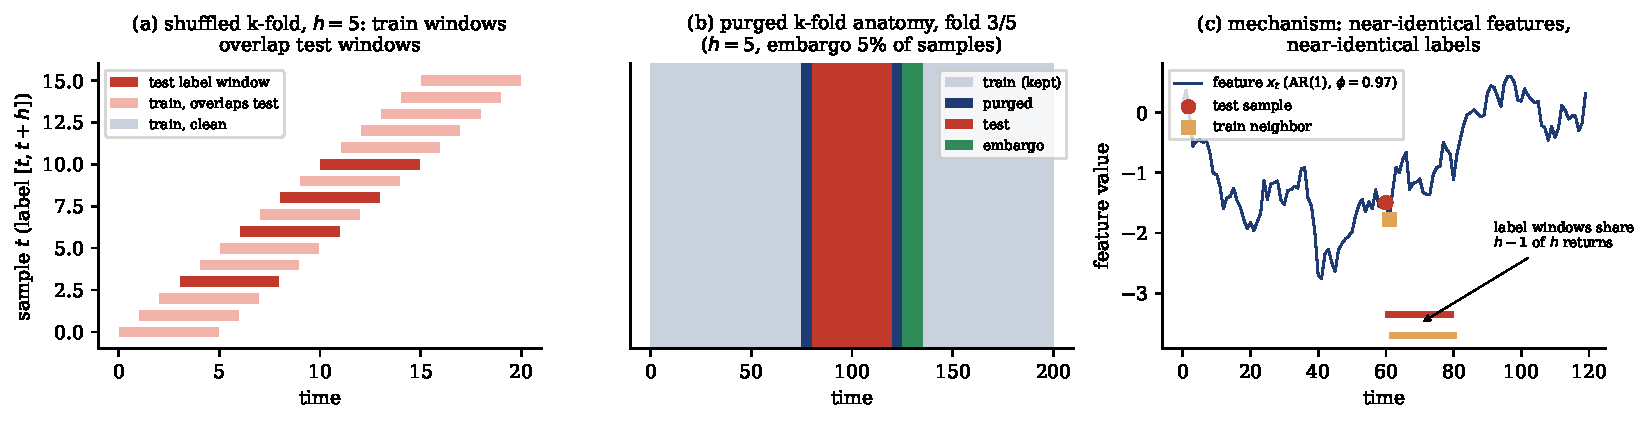
\includegraphics[width=\textwidth]{fig_setup.pdf}
\caption{The leakage anatomy, drawn by the released splitter code rather than
by hand. (a) One fold of a naive shuffled $k$-fold assignment ($16$ samples,
$k=4$, $h=5$): each bar is a sample's label window $[t, t+h]$; dark red bars
are test samples, light red bars are training samples whose windows overlap a
test window---under shuffling, overlapping training neighbors surround every
test sample. (b) Purged $k$-fold anatomy for one middle fold ($T=200$, $k=5$,
$h=5$, embargo $5\%$): the contiguous test block, the purged training samples
at both block boundaries, and the one-sided embargo after the block.
(c) The mechanism: a persistent feature (AR(1), $\phi=0.97$) is nearly
identical at a test time and its training neighbor one step later, while
their label windows share $h-1$ of $h$ returns; a flexible model can look up
the test label from a memorized training neighbor.}
\label{fig:setup}
\end{figure}

\section{Simulation framework}
\label{sec:framework}

\paragraph{Data-generating process.} Every experiment runs on a synthetic
series whose true predictability is known exactly. Returns follow
\begin{equation}
r_{t+1} \;=\; \beta\, s_t \;+\; \sigma\, \epsilon_{t+1},
\qquad \epsilon_t \stackrel{\text{iid}}{\sim} \mathcal{N}(0,1),\; \sigma = 1,
\label{eq:dgp}
\end{equation}
where $s_t$ is a latent unit-variance AR(1) signal,
$s_t = \phi_s\, s_{t-1} + \sqrt{1-\phi_s^2}\,\eta_t$. Features are of two
kinds, both AR(1) with exactly unit stationary variance. \emph{Noise
features} (five columns in the null and classification grids, four in the
signal arms) are independent
AR(1) processes with persistence $\phi$, generated independently of the
return series: their true predictive power is exactly zero, so any measured
CV skill on a noise-only configuration ($\beta = 0$) is leakage or sampling
noise. The \emph{signal feature}, present only in genuine-signal
configurations, is the latent state $s_t$ itself (optionally observed with
noise; noiselessly here). Labels are the overlapping forward sums of
Eq.~\eqref{eq:label}; a binary label $\mathbf{1}\{y_t > 0\}$ is also
produced for the classification arm. Crucially, all features are
\emph{exogenous}: none is computed from past returns. This isolates the pure
overlap channel; features derived from returns (rolling means, volatilities)
would add a second dependence channel that we deliberately exclude and
discuss in Section~\ref{sec:limitations}.

\paragraph{Closed-form population truth.} For the single-signal configuration
the population Pearson correlation between the observed feature $f_t$ and
the $h$-period label is available in closed form:
\begin{equation}
\IC_{\mathrm{pop}}
= \frac{\beta\, g_h}{\sqrt{\big(1+\nu^2\big)\big(\beta^2 V_h + h\sigma^2\big)}},
\qquad
g_h = \sum_{j=0}^{h-1}\phi_s^{\,j},
\qquad
V_h = h + 2\sum_{d=1}^{h-1}(h-d)\,\phi_s^{\,d},
\label{eq:popic}
\end{equation}
with $\nu$ the observation-noise standard deviation ($\nu = 0$ here). For
noise-only configurations $\IC_{\mathrm{pop}} = 0$ exactly. We invert
Eq.~\eqref{eq:popic} to calibrate $\beta$ so that every genuine-signal arm
has the same population IC of $0.10$ regardless of its persistence
$\phi_s$---so arms differ only in the property under study.

\paragraph{Forward-truth protocol.} Each experiment generates $T$ in-sample
observations handed to the CV schemes, followed by an $h$-step gap (so no
label window crosses the boundary), followed by $T_{\text{hold}} = 5{,}000$
forward observations that no CV procedure ever touches. For each (splitter,
model) pair we record: the \textbf{CV estimate}---the pooled out-of-sample IC
(Pearson correlation of cross-validated predictions with realized labels;
AUC for classification) exactly as a practitioner would compute it; the
\textbf{truth}---each fold's fitted model evaluated on the forward holdout,
averaged across folds; and
\begin{equation}
\text{leak} \;=\; \text{CV estimate} \;-\; \text{truth}.
\label{eq:leak}
\end{equation}
Under the null the population truth is zero (AUC: $0.5$) and the measured
forward truth is statistically indistinguishable from it, so the mean leak
in a cell is the phantom skill of that cell. Positive leak is optimism;
negative leak is pessimism, which we report but do not count as leakage to
be embargoed away. Everything is deterministic given the released seeds.

\section{Experimental setup}
\label{sec:setup}

All schemes use $k=5$ folds; the ``purged $+$ embargo'' scheme uses the
common default $\varepsilon = 2\%$ except in the embargo sweep, where
$\varepsilon$ is the design variable; walk-forward never tests the first
$40\%$. Regression models are ridge ($\alpha=1$) and a random forest ($30$
trees, depth $6$, minimum leaf $5$); classification uses logistic regression
and a random-forest classifier of the same shape. Four batches:
\begin{enumerate}\itemsep2pt
\item \textbf{Null grid} (the headline surface): noise-only configurations
crossing $h \in \{1,5,10,20\}$ with $\phi \in \{0, 0.3, 0.6, 0.9, 0.97\}$,
$16$ repetitions per cell, in-sample length $T$ drawn per repetition from
$\{800, 1600, 2400\}$, five noise features; all six splitters $\times$ both
regression models: $3{,}840$ records.
\item \textbf{Embargo sweep}: purged $k$-fold with
$\varepsilon \in \{0, 1, 2, 4, 8\}\%$ at $h=10$, $T=1600$; four
genuine-signal arms with $\phi_s \in \{0.6, 0.9, 0.97, 0.995\}$ and $\beta$
calibrated to $\IC_{\mathrm{pop}} = 0.10$ (plus four noise features,
$\phi = 0.9$), and one noise-only arm; $24$ repetitions per arm:
$1{,}200$ records. An arm is \emph{calibrated} at $\varepsilon$ if its mean
leak is $\le 0.01$ or its $95\%$ CI contains zero.
\item \textbf{Model selection}: genuine-signal configuration ($T=2000$,
$h=10$, $\phi_s = 0.97$, $\beta = 0.036$, $\IC_{\mathrm{pop}} = 0.100$, four
noise features with $\phi=0.9$) and a five-model menu---ridge, random
forests of depth $3$ and $8$, and $k$NN with $k=10$ and $k=50$. In each of
$50$ repetitions both naive and purged($+2\%$ embargo) CV score the menu and
select the argmax; every candidate's \emph{true} forward skill is measured
by refitting on all in-sample data and scoring on the holdout: $50$
records.
\item \textbf{Classification check}: noise-only configurations at $h=10$,
$T=1500$, $\phi \in \{0, 0.9\}$, $20$ repetitions, naive vs.\
purged$+$embargo, both classifiers: $160$ records.
\end{enumerate}
In total $5{,}250$ (splitter, model, series) evaluations. All intervals are
normal-approximation $95\%$ confidence intervals across repetitions. The
information coefficient is the primary metric throughout; a sign-strategy
Sharpe is recorded as a secondary descriptive metric. The Sharpe broadly
tracks the IC pattern in the product region, but it is \emph{not} a clean
interaction in the IC sense: the Sharpe of overlapping PnL has its own bias
channel, and the naive splitter shows a significant phantom Sharpe even on
the $\phi=0$ axis at long horizons (e.g.\ $+0.098\pm0.056$ at $h{=}20$,
$\phi{=}0$), so we do not rely on it for the interaction claim.

\section{Results}

\subsection{Phantom skill under the null is an interaction}
\label{sec:interaction}

Table~\ref{tab:interaction} is the headline measurement: the phantom skill
(mean leak, Eq.~\eqref{eq:leak}) of naive shuffled $k$-fold with a random
forest, on features with \emph{exactly zero} true predictive power, across
the $(h, \phi)$ grid. Figure~\ref{fig:phantom} shows the same surface
graphically alongside the other splitters.

\begin{table}[t]
\centering
\caption{Phantom skill of naive shuffled $k$-fold (random forest) under the
null: mean CV IC $-$ true forward IC, $\pm$ $95\%$ CI, $16$ repetitions per
cell. True predictive power is exactly zero everywhere in this table. The
phantom is an interaction: the $h=1$ row and the $\phi=0$ column show no
optimistic skill (two axis cells are mildly significantly \emph{negative},
consistent with the contiguity pessimism of Section~\ref{sec:embargo});
the product region is catastrophically biased. In every
cell with $h \ge 5$ and $\phi \ge 0.9$ all $16$ repetitions leak positive.}
\label{tab:interaction}
\small
\begin{tabular}{lccccc}
\toprule
& \multicolumn{5}{c}{feature persistence $\phi$}\\
\cmidrule(lr){2-6}
horizon & $0$ & $0.3$ & $0.6$ & $0.9$ & $0.97$ \\
\midrule
$h=1$  & $+0.005 \pm 0.017$ & $-0.020 \pm 0.022$ & $-0.002 \pm 0.017$ & $-0.009 \pm 0.016$ & $-0.026 \pm 0.016$ \\
$h=5$  & $-0.006 \pm 0.021$ & $+0.027 \pm 0.019$ & $+0.065 \pm 0.029$ & $+0.219 \pm 0.033$ & $+0.307 \pm 0.024$ \\
$h=10$ & $-0.020 \pm 0.016$ & $-0.008 \pm 0.018$ & $+0.075 \pm 0.030$ & $+0.298 \pm 0.033$ & $+0.465 \pm 0.040$ \\
$h=20$ & $-0.005 \pm 0.022$ & $+0.014 \pm 0.017$ & $+0.064 \pm 0.023$ & $+0.327 \pm 0.042$ & $+0.564 \pm 0.048$ \\
\bottomrule
\end{tabular}
\end{table}

Three observations. First, the \emph{interaction} is exact within sampling
noise: across the entire $h=1$ row the largest phantom skill is $+0.005$
(any $\phi$), and across the entire $\phi=0$ column the largest is $+0.005$
(any $h$). Overlapping labels with serially independent features produce
nothing---the model has no way to locate a test point's temporal neighbors,
so the shared label content is unreachable. Persistent features with
non-overlapping labels produce nothing---the neighbors are locatable but
their labels share no randomness with the test label. This is precisely the
reconciliation: the autoregressive settings in which
\citet{bergmeir2018note} prove naive CV valid, and in which
\citet{bergmeir2012use} found it empirically competitive, sit on these two
axes; the standard financial configuration ($h$-period forward labels,
persistent predictors) sits in the product region.

Second, in the product region the bias is enormous relative to any
realistic signal: $+0.307 \pm 0.024$ at $(h{=}5, \phi{=}0.97)$, rising to
$+0.564 \pm 0.048$ at $(h{=}20, \phi{=}0.97)$---an order of magnitude larger
than the information coefficients real strategies exhibit, and positive in
$16$ of $16$ repetitions in every cell with $h \ge 5$, $\phi \ge 0.9$.

Third, the leak is model-dependent in the direction the mechanism predicts:
the more local and flexible the model, the more of the leak it absorbs.
Ridge regression, which cannot memorize individual neighbors, shows roughly
one third of the random forest's phantom at the same cells ($+0.073$,
$+0.150$, $+0.182 \pm 0.044$ at $h = 5, 10, 20$ with $\phi = 0.97$). The
classification arm behaves identically in AUC units: at $\phi = 0.9$,
$h = 10$, a naive-CV random-forest classifier reports AUC $0.623$ against a
true forward AUC of $0.504$---phantom AUC $+0.119 \pm 0.010$---while
logistic regression shows $+0.042 \pm 0.014$; at $\phi = 0$ both are zero
($-0.008 \pm 0.011$ and $-0.011 \pm 0.012$), and under purged-with-embargo
CV both are slightly pessimistic everywhere ($-0.026$ to $-0.044$).

\begin{figure}[t]
\centering
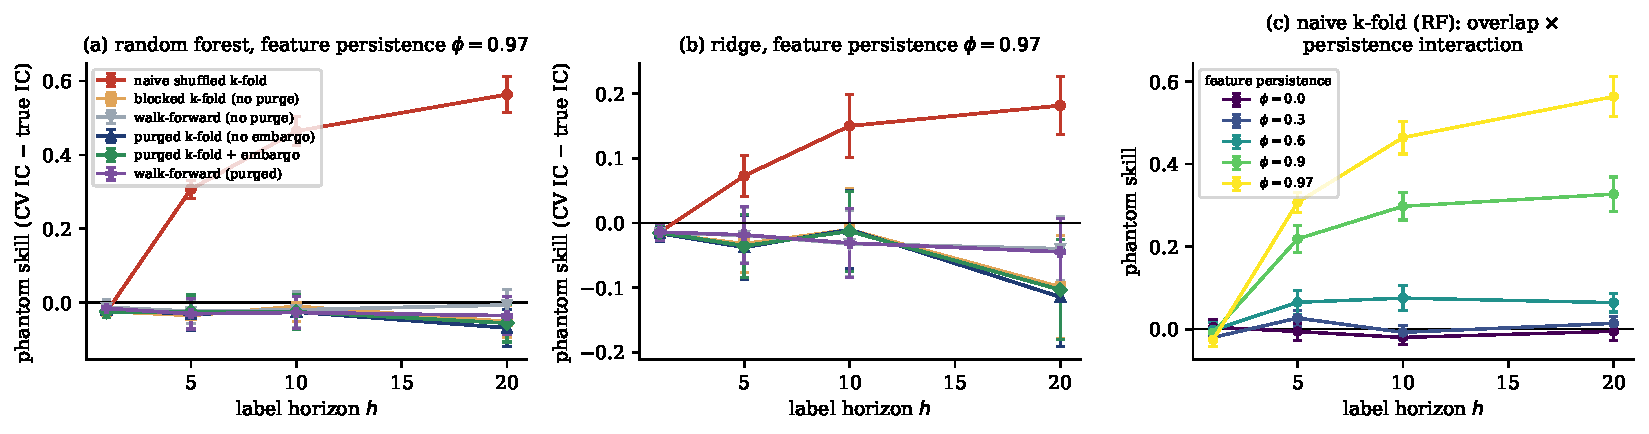
\includegraphics[width=\textwidth]{fig_phantom.pdf}
\caption{Phantom skill under the null (CV IC $-$ true forward IC; population
truth is exactly zero), $16$ repetitions per cell, error bars $95\%$ CIs.
(a) Random forest at $\phi=0.97$: naive shuffled $k$-fold rises from
${\approx}0$ at $h=1$ to $+0.56$ at $h=20$; every other splitter stays at or
below zero. (b) Ridge at $\phi=0.97$: the same shape at one third the size.
(c) The interaction, naive $k$-fold with the random forest across the full
persistence grid: the surface is flat at zero along both axes ($h=1$ or
$\phi=0$) and rises only in their product.}
\label{fig:phantom}
\end{figure}

\subsection{Blocking alone removes nearly all of the mean bias}
\label{sec:blocking}

Table~\ref{tab:splitters} compares all six splitters two ways: their worst
(most optimistic) cell anywhere on the $4 \times 5$ grid, and their leak at
the most leak-prone cell, $(h{=}20, \phi{=}0.97)$, where naive $k$-fold
shows $+0.564$.

\begin{table}[t]
\centering
\caption{Mean leak by splitter: worst (most positive) cell over the full
$(h,\phi)$ grid, and the value at the most leak-prone cell
$(h{=}20, \phi{=}0.97)$. $\pm$ are $95\%$ CIs, $n=16$ per cell. Every
non-naive splitter's worst cell occurs at $h=1$, where labels do not overlap
and the leakage mechanism is absent---i.e.\ those worst cells are sampling
noise, not residual leakage. RF $=$ random forest.}
\label{tab:splitters}
\small
\begin{tabular}{lcc@{\hskip 1.8em}cc}
\toprule
& \multicolumn{2}{c}{worst cell over grid} & \multicolumn{2}{c}{at $h{=}20$, $\phi{=}0.97$}\\
\cmidrule(lr){2-3}\cmidrule(lr){4-5}
Splitter & RF & ridge & RF & ridge \\
\midrule
naive shuffled $k$-fold       & $+0.564 \pm 0.048$ & $+0.182 \pm 0.044$ & $+0.564 \pm 0.048$ & $+0.182 \pm 0.044$ \\
blocked $k$-fold (no purge)   & $+0.004 \pm 0.019$ & $+0.008 \pm 0.024$ & $-0.052 \pm 0.043$ & $-0.099 \pm 0.079$ \\
purged $k$-fold               & $+0.009 \pm 0.019$ & $+0.008 \pm 0.024$ & $-0.069 \pm 0.050$ & $-0.115 \pm 0.076$ \\
purged $k$-fold $+$ embargo   & $+0.009 \pm 0.019$ & $+0.009 \pm 0.024$ & $-0.056 \pm 0.051$ & $-0.103 \pm 0.078$ \\
walk-forward (no purge)       & $+0.016 \pm 0.017$ & $+0.012 \pm 0.021$ & $-0.007 \pm 0.043$ & $-0.040 \pm 0.049$ \\
walk-forward purged           & $+0.015 \pm 0.015$ & $+0.012 \pm 0.021$ & $-0.036 \pm 0.051$ & $-0.045 \pm 0.052$ \\
\bottomrule
\end{tabular}
\end{table}

The result we did not expect to be this clean: \textbf{blocked $k$-fold
without any purging already removes essentially all of the mean bias}. Its
worst cell anywhere on the grid is $+0.004 \pm 0.019$ (RF) and
$+0.008 \pm 0.024$ (ridge)---both at $h=1$, where no overlap exists, i.e.\
sampling noise---and at the cell where naive CV hallucinates $+0.564$,
blocking alone shows $-0.052 \pm 0.043$. The arithmetic explains why: with
contiguous test blocks, overlapping train/test pairs survive only within $h$
samples of the two block boundaries, a $O(h/T)$ fraction of pairs, versus
$O(1)$ under shuffling. At $h \ll T$ the surviving boundary leak is
second-order in the mean. Unpurged walk-forward behaves the same way
($+0.016$ worst, one boundary per fold). What purging changes in the mean,
at these horizons, is statistically nothing; what it changes structurally is
the \emph{guarantee}---the exhaustive pair checker certifies zero
overlapping pairs, for any $h$, any fold geometry, any future configuration
in which $h$ is not small relative to the block length. We state this
honestly as the paper's mildly contrarian finding: at $h \ll T$, contiguity
does the calibration work, and purging is cheap insurance on the worst
case rather than a correction of the average.

The residuals of all contiguous schemes at high $(h,\phi)$ are
\emph{negative}: blocked, purged, and embargoed $k$-fold sit between
$-0.05$ and $-0.12$ at $(h{=}20, \phi{=}0.97)$. This is contiguous-fold
pessimism, not residual leakage: with strongly overlapping labels a test
block contains few effectively independent label windows, and a model fit
outside the block regresses toward its own training period, so the pooled CV
correlation systematically underestimates the same models' forward skill on
a long holdout. Two caveats scope this. First, the magnitude is specific to
the \emph{pooled-prediction} convention we adopt as ``what a practitioner
computes'': scoring each fold's IC separately and averaging shrinks the
pessimism substantially, because much of it comes from pooling predictions
across heterogeneous contiguous folds rather than from the splits
themselves. Second, the direction is what matters for practice: the honest
procedure does not merely remove the optimism; under the pooled convention it
leaves an estimate that is, if anything, slightly conservative---a property
practitioners should budget for (or sidestep by fold-averaging) rather than
``fix'' by un-purging.

\subsection{Purging is calibrated at zero embargo; the embargo bought nothing here}
\label{sec:embargo}

The embargo sweep asks the textbook question directly: after purging, how
much embargo is required before residual CV optimism disappears? In this
design the answer is \textbf{none, in every arm}
(Figure~\ref{fig:embargo}). At $\varepsilon = 0$, all ten (arm, model)
combinations---four genuine-signal persistence levels up to
$\phi_s = 0.995$ plus the null arm, each under both models---already meet
the calibration criterion. The residual leak at zero embargo ranges from
$-0.010$ to $-0.102$: every single one is \emph{negative} (the
contiguous-fold pessimism of Section~\ref{sec:blocking}), so there is no
optimism left for an embargo to remove. And the sweep is flat: across the
entire grid $\varepsilon \in \{0, 1, 2, 4, 8\}\%$, the largest within-arm
movement of the mean residual is $0.012$, far inside every confidence
interval. The cost side, by contrast, is real and linear: the purge alone
discards $1.2\%$ of training candidates at this geometry ($h=10$,
$T=1600$, $k=5$), and the $8\%$ embargo discards $9.2\%$
(Figure~\ref{fig:embargo}c).

We disclose the scope of this negative result plainly rather than
generalize it. Our features are exogenous AR(1) processes: their serial
dependence does not involve the return series, so once label-window overlap
is purged, nothing in the training set echoes the test labels. The embargo
exists for a different case---features \emph{derived from} past returns
(rolling means, realized volatilities, momentum), whose values shortly after
the test block mechanically contain the test block's returns even though
their label windows do not intersect it. That channel is absent from this
design by construction, and our experiments say nothing about it; we flag it
as the natural follow-up (Section~\ref{sec:limitations}). What the
experiments do establish is the converse caution: the common reflex of
applying a fixed $1\%$--$2\%$ embargo as a default tax is not supported by
the overlap mechanism itself, even at signal persistence $0.995$---if an
embargo is justified, it is justified by return-derived features, and its
size should be measured, not assumed.

\begin{figure}[t]
\centering
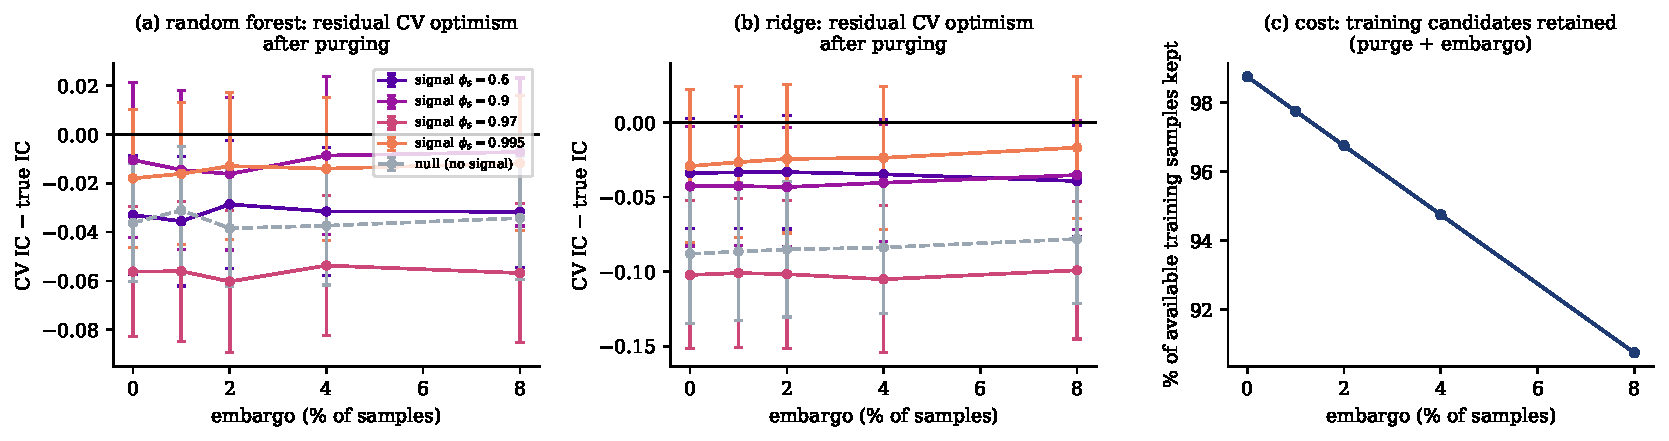
\includegraphics[width=\textwidth]{fig_embargo.pdf}
\caption{The embargo sweep: residual leak of purged $k$-fold as the
one-sided embargo grows from $0$ to $8\%$ of the sample ($h=10$, $T=1600$,
$24$ repetitions per arm, $95\%$ CIs). (a) Random forest and (b) ridge:
four genuine-signal arms (signal persistence $\phi_s = 0.6$--$0.995$, each
calibrated to population IC $0.10$) and the null arm (dashed). Every arm is
calibrated already at zero embargo; the residual is negative
(contiguous-fold pessimism) and the curves are flat---the embargo buys
nothing in this design. (c) Its cost is real: training candidates retained
fall linearly from $98.8\%$ (purge only) to $90.8\%$ at an $8\%$ embargo.}
\label{fig:embargo}
\end{figure}

\subsection{What purging costs}
\label{sec:costs}

Table~\ref{tab:costs} prices the honest procedures on the null grid. Purged
$k$-fold retains $98.7\%$ of available training candidates (the null grid
averages over $h$ up to $20$ and $T$ down to $800$, where the purge share is
largest; at the embargo sweep's geometry it is $98.8\%$), and the default
$2\%$ embargo lowers retention to $96.7\%$. The dispersion price of honesty
is visible but modest: the repetition-level standard deviation of the CV
estimate rises from $0.048$ (naive, RF) to $0.058$ for purged $k$-fold,
$+21\%$ (repetitions randomize $T \in \{800, 1600, 2400\}$, so these are
dispersions over a mixture of sample sizes; the cross-splitter comparison is
unaffected since every splitter sees the same series). The decomposition
matters: blocked $k$-fold without purging already
shows $0.057$, so almost the entire dispersion increase is the price of
\emph{contiguity}---fewer effectively independent label windows per
fold---and the purge itself adds about one percent. Walk-forward is the
expensive option: it trains on $72.7\%$ of the available candidates on
average (the early folds see far less) and its fold-level dispersion is
about twice naive $k$-fold's ($0.050 \to 0.104$), the familiar price of
evaluating only on late, single-pass blocks.

\begin{table}[t]
\centering
\caption{Costs on the null grid ($320$ records per cell): fraction of
available training candidates retained (identical for both models), the
across-fold standard deviation of the fold-level CV estimate, and the
across-repetition standard deviation of the pooled CV estimate within an
$(h,\phi)$ cell, averaged over cells.}
\label{tab:costs}
\small
\begin{tabular}{lc@{\hskip 1.8em}cc@{\hskip 1.8em}cc}
\toprule
& & \multicolumn{2}{c}{random forest} & \multicolumn{2}{c}{ridge}\\
\cmidrule(lr){3-4}\cmidrule(lr){5-6}
Splitter & train kept & fold std & rep.\ std & fold std & rep.\ std \\
\midrule
naive shuffled $k$-fold       & $100.0\%$ & $0.050$ & $0.048$ & $0.050$ & $0.053$ \\
blocked $k$-fold (no purge)   & $100.0\%$ & $0.074$ & $0.057$ & $0.084$ & $0.077$ \\
purged $k$-fold               & $98.7\%$  & $0.074$ & $0.058$ & $0.084$ & $0.077$ \\
purged $k$-fold $+$ embargo   & $96.7\%$  & $0.073$ & $0.059$ & $0.084$ & $0.077$ \\
walk-forward (no purge)       & $72.7\%$  & $0.104$ & $0.054$ & $0.122$ & $0.066$ \\
walk-forward purged           & $72.0\%$  & $0.105$ & $0.057$ & $0.123$ & $0.067$ \\
\bottomrule
\end{tabular}
\end{table}

\subsection{Model selection: where the bias becomes a wrong decision}
\label{sec:selection}

A biased estimate is survivable; a biased \emph{choice} is not. The
selection batch puts a genuine signal in the data (population IC $0.100$)
and lets each CV scheme choose from a five-model menu whose true forward
skills we measure exactly. Table~\ref{tab:selection} and
Figure~\ref{fig:selection} report the outcome.

\begin{table}[t]
\centering
\caption{Model selection with a genuine signal (population IC $0.100$, $50$
repetitions, $\pm$ $95\%$ CIs). ``True IC'' is the selected model's forward
holdout IC after refitting on all in-sample data; optimism $=$ CV claim $-$
true; regret $=$ oracle true IC $-$ selected true IC. The five-candidate
menu's true forward ICs: ridge $0.059 \pm 0.014$, RF depth~3
$0.041 \pm 0.011$, RF depth~8 $0.027 \pm 0.010$, $k$NN($50$)
$0.021 \pm 0.009$, $k$NN($10$) $0.012 \pm 0.008$.}
\label{tab:selection}
\small
\begin{tabular}{lcccc}
\toprule
 & CV IC of pick & true IC of pick & optimism & regret \\
\midrule
naive shuffled $k$-fold & $0.422 \pm 0.011$ & $0.012 \pm 0.008$ & $+0.410 \pm 0.012$ & $0.056 \pm 0.011$ \\
purged $+$ embargo      & $0.053 \pm 0.019$ & $0.042 \pm 0.013$ & $+0.012 \pm 0.020$ & $0.027 \pm 0.008$ \\
oracle                  & ---               & $0.069 \pm 0.012$ & ---                & $0$ \\
\bottomrule
\end{tabular}
\end{table}

Naive CV does not merely overstate the chosen model's skill---it chooses the
\emph{wrong model, every time}. In $50$ of $50$ repetitions it selects
$k$NN with $k=10$, the most local model in the menu and, by the mechanism of
Section~\ref{sec:interaction}, the best leakage harvester: with persistent
features, a test point's nearest neighbors in feature space \emph{are} its
temporal neighbors, whose overlapping labels contain the answer. The same
locality that maximizes the leak makes it the menu's \emph{worst} true model
(forward IC $0.012$, against ridge's $0.059$). Naive CV claims $0.422$ for
this pick; its true skill is $0.012$---an optimism of $+0.410$. (A small
part of any CV-vs-truth optimism is a benign train-size effect---CV models
train on $4/5$ of the data while the truth refits on all of it---but that
effect is shared by every splitter and is dwarfed here by the leakage term.)
Under
leakage, CV ranks models by their capacity to exploit the leak, which here
is anti-correlated with true skill.

Purged CV repairs the decision, not just the number. It picks the truly
best candidate (ridge) most often ($23/50$), distributes the rest across the
menu ($\text{RF}_{d8}$ $9$, $k$NN$_{10}$ $9$, $k$NN$_{50}$ $5$,
$\text{RF}_{d3}$ $4$), claims $0.053$ where the truth is $0.042$ (optimism
$+0.012 \pm 0.020$, indistinguishable from zero), and cuts regret in half
($0.056 \to 0.027$ against an oracle of $0.069$). The end-to-end payoff,
the only number a practitioner ultimately cares about: switching the
selection procedure from naive to purged CV raises the deployed model's true
forward IC by $+0.029 \pm 0.012$, with purged winning in $64\%$ of
repetitions, tying in $18\%$, and losing in $18\%$. On a population signal
of $0.100$, the choice of validation scheme is worth more than a quarter of
the signal itself.

\begin{figure}[t]
\centering
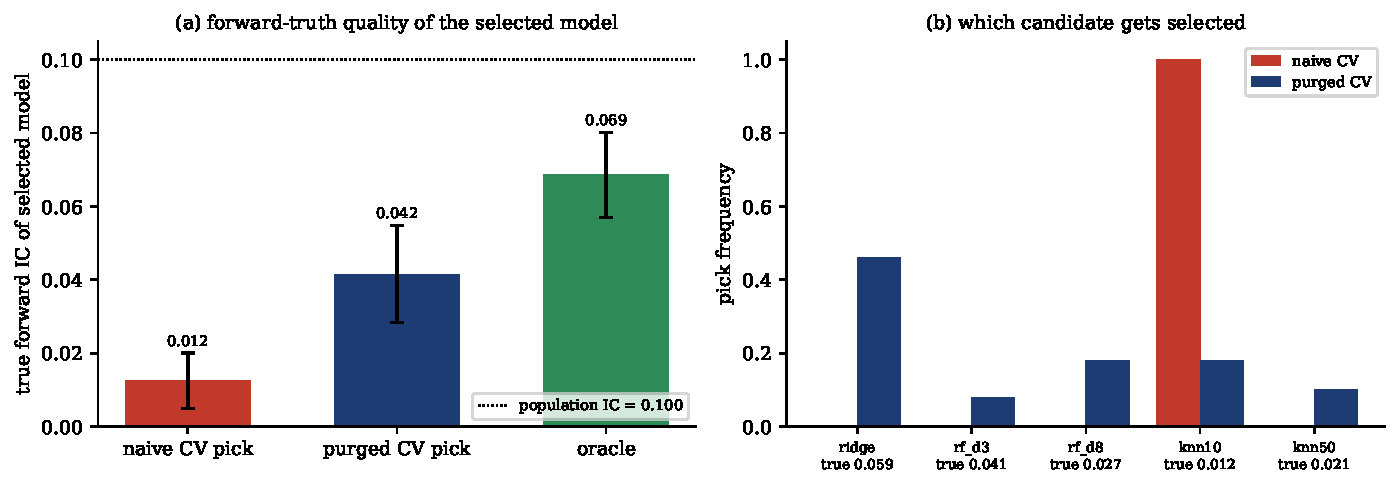
\includegraphics[width=0.92\textwidth]{fig_selection.pdf}
\caption{Model selection with a genuine signal (population IC $0.100$,
dotted line; $50$ repetitions; $95\%$ CIs). (a) True forward IC of the model
each procedure selects: naive CV $0.012$, purged CV $0.042$, oracle
$0.069$. (b) Pick frequencies; tick labels carry each candidate's measured
true forward IC. Naive CV picks $k$NN($10$)---the menu's truly worst model
but its best leakage harvester---in $50$ of $50$ repetitions; purged CV
picks ridge, the truly best, most often ($46\%$).}
\label{fig:selection}
\end{figure}

\section{Discussion}
\label{sec:discussion}

\paragraph{The reconciliation.} The two literatures that motivated this
study are both right, about different regimes, and the experiment locates
the boundary. \citet{bergmeir2018note}'s validity result and the empirical
pro-CV findings \citep{bergmeir2012use,cerqueira2020evaluating} concern
settings that live on the axes of Table~\ref{tab:interaction}: one-step
labels (no overlap) or, more generally, no mechanism by which a model can
look up a test sample's label content from training points. The
financial-ML warnings \citep{lopezdeprado2018advances} concern the product
region: multi-period forward labels \emph{and} features persistent enough to
index temporal neighborhoods. Neither overlap nor persistence alone is
dangerous; their product is, and it grows quickly ($+0.31$ already at
$h=5$, $\phi=0.97$ for a flexible model). The practical diagnostic is
correspondingly simple: count overlapping train/test label-window pairs
(our released checker does exactly this) and ask whether any feature is
persistent enough to act as an index. If either answer is ``no,'' naive CV's
mean is fine in this mechanism's terms; if both are ``yes,'' it is not---and
no amount of averaging over folds will save it, since the bias is positive
in every repetition.

\paragraph{A practical recipe.} The decomposition in
Sections~\ref{sec:blocking}--\ref{sec:costs} supports an ordered
prescription. (i) \emph{Always use contiguous folds.} Blocking is free---no
data discarded---and removes nearly all of the mean bias; shuffled folds on
overlapping labels are indefensible. (ii) \emph{Purge for the guarantee.}
At $h \ll T$ purging changes the mean estimate by approximately nothing,
but it costs only $1.2\%$ of training candidates and converts ``small by
arithmetic'' into ``zero by construction''---insurance that becomes load-bearing
exactly when $h$ grows relative to the fold length, where the boundary
arithmetic stops being second-order. For model \emph{selection}, use purged
CV unconditionally: that is where the bias becomes a wrong decision and
where we measure the payoff ($+0.029$ forward IC). (iii) \emph{Treat the
embargo as a measured response to return-derived features, not a default
tax.} In our design---exogenous features, the pure overlap channel---zero
embargo left no residual optimism in any of the ten arms, and signal persistence up to
$0.995$ did not change that. The embargo's justification is a different
channel (features computed from returns echoing the test block), which we
did not test; if your features are return-derived, measure the required
embargo rather than assuming $1\%$. (iv) \emph{Budget for pessimism.}
Honest contiguous CV under heavy overlap reads low ($-0.01$ to $-0.10$ in
our arms) relative to true forward skill, and its dispersion is ${\sim}20\%$
higher---costs of contiguity, not of purging. A practitioner comparing an
honest pipeline against a remembered naive baseline should expect the
honest number to look worse twice over: the phantom is gone, and the
estimator is conservative.

\paragraph{Why the selection result is the important one.} Estimation bias
can in principle be discounted by a sufficiently skeptical reader; selection
bias cannot, because it changes which model exists downstream. The
mechanism is adversarial in the precise sense that the leak is not noise
added to all candidates equally---it is a reward for memorization capacity,
so CV under leakage \emph{sorts} the menu by the wrong criterion. Our menu
makes this stark (the truly worst model wins $50/50$), but the logic is
general: any hyperparameter that controls locality or capacity (tree depth,
$k$, bandwidth, attention window) will be pushed toward the
leakage-maximizing end by naive CV on overlapping labels. This connects the
split-induced channel measured here to the selection-induced channel of
\citet{bailey2014pseudo,bailey2017probability}: leaky validation scores are
exactly the kind of inflated, correlated trial statistics that
multiple-testing corrections assume away.

\section{Limitations}
\label{sec:limitations}

Our features are \emph{exogenous} AR(1) processes; no feature is computed
from past returns. This isolates the overlap channel cleanly but excludes
the channel that motivates the embargo---return-derived features (rolling
statistics of returns) whose post-test values mechanically contain test-block
information. Our embargo-bought-nothing result therefore delimits, and does
not refute, the embargo; testing the return-derived case with the same
forward-truth protocol is the natural next experiment. Return innovations
are Gaussian and i.i.d.; volatility clustering, fat tails, and regime
shifts would interact with both the leak and the pessimism in ways we do
not measure. Horizons satisfy $h \ll T$ ($h/T \le 2.5\%$); when label
windows are long relative to fold length, blocking's boundary arithmetic
stops being second-order, and purging's \emph{mean} contribution should
grow---our claim that blocking suffices in the mean is a claim about the
tested regime, not a theorem. The model set is small and standard (ridge,
random forests, $k$NN, logistic); the leak's magnitude is model-dependent,
and more aggressive memorizers (boosting, nearest-neighbor ensembles, deep
networks) plausibly absorb more. The calibration criterion involves a
threshold ($0.01$) and a CI rule, both disclosed and fixed before the
sweep. Finally, the population IC is derived in closed form only for a
single signal feature, which is why the genuine-signal arms carry one; the
IC is the primary metric throughout, with the sign-strategy Sharpe recorded
as a secondary check.

\section{Conclusion}

We measured, against known ground truth, how much of financial machine
learning's purging prescription is load-bearing. The leakage it targets is
real and large, but it is an \emph{interaction}: overlapping forward labels
and persistent features jointly produce phantom CV skill up to
$+0.56$ IC under an exact null, while either ingredient alone produces
none---which reconciles the textbook warning of
\citet{lopezdeprado2018advances} with the validity results of
\citet{bergmeir2018note}; each describes one regime of the same surface.
Of the remedy's three components, contiguous folds do nearly all of the
mean-bias work at $h \ll T$; purging costs $1.2\%$ of the training data and
upgrades the arithmetic to a guarantee of zero overlapping pairs; the
embargo, for exogenous features, bought nothing at any tested persistence
---a negative result we report with its scope, since return-derived features
are the case it exists for and remain untested here. The unambiguous payoff
of purged CV is decisional: under leakage, cross-validation ranks models by
their capacity to exploit the leak, selecting the truly worst candidate in
$50$ of $50$ trials; purging restores honest selection and lifts deployed
forward skill by $+0.029 \pm 0.012$ on a $0.100$ signal. Use contiguous
folds always; purge for the guarantee and for every selection decision;
embargo when---and by how much---your features, not your habits, require it.

\paragraph{Reproducibility.} All experiments are deterministic given the
released seeds. A single command (\texttt{python scripts/run\_all.py})
regenerates every record and summary statistic---the file
\texttt{results/results.json} and four per-record CSV files---and the
package's figures module regenerates every figure from those results; a
companion script (\texttt{scripts/check\_paper\_numbers.py}) asserts that
every number quoted in this paper matches the generated results. The
splitters are implemented
from scratch, and the test suite includes an exhaustive proof that the
purged splitters produce zero overlapping train/test label-window pairs on
every tested configuration. The data-generating process, splitters,
evaluation harness, and analysis are provided as an open-source package.

\small
\bibliographystyle{plainnat}
\bibliography{refs}

\end{document}
